%        File: intro.tex
%     Created: Thu Jun 22 04:00 PM 2017 E
% Last Change: Thu Jun 22 04:00 PM 2017 E
%
% arara: pdflatex: {options: "-draftmode"}
% arara: biber
% arara: pdflatex: {options: "-draftmode"}
% arara: pdflatex: {options: "-file-line-error-style"}
\documentclass[MilwayThesis]{subfiles}

\begin{document}
This thesis asks a seemingly simple question: Why do some but not all languages allow their users to generate adjectival resultatives?
I write ``\textit{seemingly} simple'' for reasons that are likely obvious to anyone reading this, but will clarify the reasons as a way of introducing the content of the thesis that follows.
There are, as far as I can tell, two complications inherent in questions of the form \textit{Why P?}: one linguistic, one metaphysical.
The linguistic complication is that \textit{Why P?} presupposes that \textit{P}.
In order to even be justified in asking the question posed above, then, we must first demonstrate that there is a class of expressions that can be called adjectival resultatives, and that they are not found in every language.
The metaphysical complication is due to the fact that a given \textit{Why} question has an indefinite number of true responses, yet the appropriate response depends on the level of explanation that is sought.
So, in order to answer the question, we must clarify the level of explanation we are seeking.

Beginning with the presupposition: is it the case that some but not all natural language grammars generate adjectival resultatives?
The first thing we need to answer that question is a working definition of adjectival resultatives, which I give in \cref{def:AdjRes} and which, in turn, depends on the definition of \textit{secondary predicate} in \cref{def:SecPred}.
\begin{defn}[Adjectival Resultative]\label{def:AdjRes}
	An \textit{adjectival resultative} is a secondary predication structure, whose secondary predicate is an adjective (phrase) and is interpreted as describing a state directly caused by the event described by the primary predicate.
\end{defn}
\begin{defn}[Secondary Predication]\label{def:SecPred}
	A \textit{secondary predication} structure is a monoclausal structure containing a constituent consisting of a verb (phrase) (V) an argument (DP) and another element (SP) such that, SP is interpreted as a predicate, and DP is an argument of both V and SP.
\end{defn}

A canonical example of an adjectival resultative is give in \cref{ex:AREx}.
\ex. \label{ex:AREx} Natalie hammered the metal flat.

This is a secondary predication structure in the sense that it contains a constituent \textit{hammer the metal flat} which contains a verbal and an adjectival predicate (\textit{hammer} and \textit{flat}, respectively) and a DP \textit{the metal} which is an argument of both predicates.
Furthermore, it is an adjectival resultative because its secondary predicate is the adjective \textit{flat}, which describes a state caused by the hammering event.
Resultatives contrast minimally with depictives, like the one in \cref{ex:DepictiveCanon}---secondary predication structures whose secondary predicate describes a state not caused by the primary predicate.
\ex.\label{ex:DepictiveCanon} Heather ate the fish raw.

This is an example of secondary predication, with \textit{ate} being the verb, \textit{raw} being the secondary predicate, and the argument \textit{the fish} shared between the two.
It is not a resultative because, in the situation it describes, the rawness state is not caused by the eating event.
So, part of the presupposition is true: resultatives exist in at least one language.
\textcite{snyder1995language,snyder2001nature} demonstrates that adjectival resultatives exist in a number of other languages, including ASL, Dutch, German, Khmer, Japanese, Korean, Hungarian, Mandarin, and Thai.
\ex. Examples of adjectival resultatives\footnote{Unless otherwise noted, these examples are drawn from \textcite{snyder2001nature}}
\a. J-O-H-N PAINT CHAIR RED\hfill\parencite[ASL,][]{kentner2018wh}\\
``John painted the chair red.''
\bg. Hans h\"ammert das Metall flach.\\
Hans hammered the metal flat\\
``Hans hammered the metal flat.'' \hfill \raisebox{1.4\baselineskip}[0pt][0pt]{(German)}
\bg. A munk\'as lapos-ra kalap\'acsolta a f\'emet.\\
the worker flat-\textsc{trans} hammer-\textsc{pst} the metal\\
``The worker hammered the metal flat.''\rcommentg{(Hungarian)}
\bg. John-ga teeburu-o kiree-ni hui-ta.\\
John-\textsc{nom} table-\textsc{acc} clean wipe-\textsc{pst}\\
``John wiped the table clean.''\rcommentg{(Japanese)}
\bg. Kira wai daik kpaet.\\
Kira hit metal flat\\
``Kira beat the metal flat.''\rcommentg{(Khmer)}
\bg. John-i teibl-ul kekuti tak-at-ta\\
John-\textsc{nom} table-\textsc{acc} clean polish-\textsc{pst}-\textsc{comp}\\
``John wiped/polished the table clean.''\rcommentg{(Korean)}
\bg. Ta ba tie guan da ping.\\
(s)he \textsc{ba} iron pipe hit flat\\
``(S)he beat the iron pipe flat.''\rcommentg{(Mandarin [tones omitted])}
\bg. Ja: t'up lo:ha\textglotstop{} haj bae:n\\
\textsc{neg-imper} hammer metal \textsc{haj} (be-)flat\\
``Don't hammer the metal flat.''\rcommentg{(Thai [tones omitted])}
\bg. Sahar kota ban asen saf (gard chakosh)\\
Sahar hit.\textsc{pst} on iron flat with hammer\\
``Sahar pounded the iron flat (with a hammer).''\rcommentg{(Southern Kurdish, Koorosh Ariyaee p.c.)}

Furthermore, Snyder demonstrates that some languages seem to be incapable of generating adjectival resultatives, expressing resultatives periphrastically instead.
\ex. Examples of periphrastic resultative.\footnote{These examples are drawn from \textcite{snyder2001nature} unless otherwise noted.}
\ag. Lokoda taroktu el hadide haete\textglotstop{} osbohoh mosoto\textglotstop{}han.\\
Lokoda beat the metal/iron until it.became flat\\
``Lokoda beat the metal \textit{until it became} flat''\rcommentg{(Arabic, Egyptian)}
\bg. Gorri-z atz-azal-ak pintatzen ari naiz\\
red-with/in finger.covering-\textsc{pl} painting \textsc{aux}\\
``I am painting my finger nails \textit{with/in} red.''\rcommentg{(Basque)}
\bg. Jean a martel\'{e} le m\'{e}tal jusqu'\`{a} ce qu'il \'{e}tait plat\\
John has hammered the metal until-to that that-it be.\textsc{pst} flat\\
``John hammered the metal until it was flat.''\rcommentg{(French)}
\bg. Dani tzavaA \textglotstop{}it ha-bayet bi-\textglotstop{}adoom.\\
Dani painted P(\textsc{acc}) the-house in-red\\
``Dani painted the house \textit{in} (the colour) red.''\rcommentg{(Hebrew, Modern)}
\bg. $\left[\text{Tukang pande-nipun}\right]$ mande wesi ngantos gepeng.\\
{worker forge-\textsc{poss}} beat iron until flat\\
``The blacksmith beat the iron \textit{until} (it was) flat.''\rcommentg{(Javanese)}
\bg. Joe abisi ndako na modobo motani.\\
Joe he.paint house with paint red\\
``Joe painted the house \textit{with} red paint.''\rcommentg{(Lingala)}
\bg. Ivan pokrasil dom v krasnyj tsvet.\\
John paint.\textsc{pst} house in red colour\\
``John painted the house \textit{in} the color red''\rcommentg{(Russian)}
\bg. John je ofarbao kucu u crveno.\\
John is painted house in red\\
``John painted the house \textit{in} (the colour) red.''\rcommentg{(Serbo-Croatian)}
\bg. Juan golpe\'{o} el hierro hasta que estaba plano.\\
John beat.\textsc{pst} the iron until that be.\textsc{pst} flat\\
``John beat the iron \textsc{until} it was flat.''\rcommentg{(Spanish)}

Our presupposition, then, seems to hold; some, but not all languages exhibit adjectival resultatives.

Our second issue---that of deciding what we mean by \textit{why}---I believe is a far more interesting one, as answering it requires us to be explicit about the broader goals of our inquiry.
If our interest is historical linguistics or language variation and change, then we might be interested in migration patterns and language contact situations, and how they do or do not correlate with a language's ability to generate resultatives, or with the social factors linked to resultatives.
This thesis, however, is a work of largely theoretical generative syntax, so our \textit{why} question is actually two questions: What essential property or properties do grammars that generate resultatives have, that grammars that do not generate resultatives lack? And how is that property or set of properties acquirable by children from the primary linguistic data?
Note that I have framed the acquisition question as dependent on the grammatical question---likely a reflection of my training as a syntactician---but I don't believe that one question is \textit{logically} prior to the other.
\textcite{snyder1995language,snyder2001nature}, for instance, takes the grammatical question to be dependent on the acquisition question.
I believe the questions are interdependent, meaning that the correct answer to one should at least be consistent with the correct answer to the other.
The simplest situation, however, would be that the correct answer to each question entails the correct answer to the other; in other words, that a single statement would provide an answer to both questions.

For reasons that have little to do with the content of linguistic theory or its empirical base, and a great deal to do with the social, cultural, and political atmosphere of modern scientific research, the two questions that I pose above are not commonly treated as interdependent.
Syntacticians tend to focus on the grammatical question, and consider the acquisition question to be secondary at best, while acquisitionists tend to consider the reverse to be the case.
This leads to syntactic proposals where the acquisition question is ignored or treated as an afterthought, and acquisition studies which do not fully address how their results could be integrated into linguistic theory.
With this thesis, I hope to avoid this pitfall.
That is, I aim to develop a theoretical explanation of the resultative parameter that takes the acquisition question to be a crucial criterion for the success of my proposal; in other words, I assume that a grammatical theory of resultatives is adequate only if it answers the acquisition question.
This statement is likely uncontroversial among generative syntacticians; indeed it is perhaps an unstated criterion of all generative syntax.
I make it a stated criterion here as a way of ensuring that readers can hold me to it.

The answer I will argue for here is that a grammar generates resultatives only if it also generates adjectives without $\varphi$-features.
I argue that this parameter is both acquirable and consistent with Snyder's results.
Since $\varphi$-features on adjectives manifest themselves as agreement morphology, their presence or absence is directly detectable, and therefore acquirable.
The demonstration that Snyder's results can be derived from the presence or absence of $\varphi$-features on adjectives, however, is highly technical, based on a non-standard version of so-called minimalist theory.
In \cref{sec:nonstandard}, I argue that the non-standard aspects of the theory I assume, in fact, follow from entirely standard assumptions in contemporary syntactic theory, which I discuss in detail in \cref{sec:standard}.
With these assumptions---standard and non-standard---in place, I assess the current syntactic analyses of adjectival resultatives in \cref{sec:litreview} before synthesizing these analyses into my own analysis in \cref{sec:analysis}.
The analysis that I settle on, shown in \cref{fig:ResStructIntro}, is modified from that of \textcite{kratzer2004building}.
\begin{figure}[h]
	\centering
	{\small
\begin{forest}
    nice empty nodes,sn edges,baseline,
%    for tree={
%    calign=fixed edge angles,
%    calign primary angle=-30,calign secondary angle=60}
    [VP
	    [VP
		    [hammer]
		    [DP[the metal,roof,name=compV]]
	    ]
	    [resP
		    [$\langle$DP$\rangle$,name=specRes]
		    [
			    [res]
			    [SC
				    [$\langle$DP$\rangle$,name=SCDP]
				    [
					    [adj]
					    [\textsc{flat}]
				    ]
			    ]
		    ]
	    ]
    ]
    \draw[->] (SCDP) to[out=south west, in=south] (specRes);
    \draw[->] (specRes) to[out=south, in=south east] (compV);
\end{forest}
}
\caption{The structure of resultatives proposed in \cref{sec:analysis}}
	\label{fig:ResStructIntro}
\end{figure}
Note three non-standard properties of this analysis: resP is adjoined to VP, the shared argument \textit{the metal} undergoes sideward movement, and that movement is into a $\theta$-position.
These properties will be explained in a principled manner throughout the thesis.

Before my ultimate explanation of the resultative parameter, in \cref{sec:labels}, I introduce and discuss label theory \parencite{chomsky2013problems,chomsky2015problems},  a new modification to minimalist syntactic theory.
Finally, in \cref{sec:deriving} I show how the assumptions, hypotheses, and analyses that I mention above allow me to derive Snyder's (\citeyear{snyder2016compound}) correlation between resultatives and bare stem compounding.

While this derivation, which ends \cref{sec:part1} of this thesis, might seem to fully explain the resultative parameter, and therefore fulfill the stated goal of my thesis, I go on in \cref{sec:part2} to consider the broader implications of the account I give in \cref{sec:part1}.
For instance, my account of the resultative parameter seems to be too strong, eliminating the possibility of expressions derived from small clauses in languages which do not have resultatives.
That is, my account would seem to predict that a language like French would fail to generate copular clauses and depictives like the examples in \cref{ex:FreCopIntro} and \cref{ex:FreDepIntro}, respectively.
\exg. \label{ex:FreCopIntro}Jeanne est grand -e.\\
Jeanne is tall -FSg\\
``Jeanne is tall.''

\exg. \label{ex:FreDepIntro}Marie mange la viande crue\\
Marie eats the.FSg meat raw.Fsg\\
``Marie eats meat raw''

In \cref{sec:FreSC}, however, I propose a refinement of the grammatical architecture which places the operation Agree outside the narrow syntax, before Label, and show that this proposal eliminates the faulty prediction made in \cref{sec:part1}.

\Cref{sec:ACCing} discusses a puzzling aspect of the structure I propose for resultatives (see \cref{fig:ResStructIntro})---namely, the fact that sideward movement from [Spec, res] to [Comp, V] seems to be obligatory.
I highlight the puzzling nature of this by discussing the analysis of ACC-ing clauses given by \textcite{cinque1996pseudo}, in which such sideward movement is also obligatory.
In order to explain these analyses, I make two modifications to Chomsky's label theory, modifications which I argue are independently motivated.
I then show that obligatory sideward movement follows from the resulting version of label theory.

Finally, in \cref{sec:coincidence}, I discuss the interpretation of resultatives and constructions with similar structures (depictives and some ACC-ing constructions).
I argue that given the right theory of event semantics, these structures with such seemingly different interpretations are, in fact, very similar.
They are all species of secondary predication structures in which the primary and secondary predicates take the same eventuality (or situation) argument.
\section{Theoretical Context}\label{sec:standard}
The general theory that I assume here is a variety of what is called \textit{minimalist syntax} after Chomsky's (\citeyear{chomsky1995minimalist}) \textit{The Minimalist Program}.
Using the term \textit{minimalism} to refer to a theory of grammar, however, is perhaps incorrect, as minimalism is a metatheoretical position.
The contrast between theory and metatheory that I assume here is due to \textcite{chametzky1996theory}\footnote{
	Chametzky makes a three-way distinction between metatheoretical, theoretical, and analytic work:
	\begin{quote}
		\textit{Metatheoretical} work is theory of theory, and divides into two sorts: general and (domain) specific.
		\textit{General} metatheoretical work is concerned with developing and investigating adequacy conditions for any theory in any domain.
		So, for example, it is generally agreed that theories should be (1) consisted and coherent, both internally and with other well-established theories; (2) explicit; and (3) simple. This sort of work is philosophical in nature [\ldots].
		\textit{Specific} metatheoretical work is concerned with adequacy conditions for theory in a particular domain.
		So, for example, in linguistics	we have Chomsky's (1964; 1965) familiar distinctions among observational, descriptive, and explanatory adequacy.
		Whether such work is ``philosophy'' or, in this case, ``linguistics'' seems to me a pointless question.
		
		\textit{Theoretical} work is concerned with developing and investigating primitives, derived concepts, and architecture within a particular domain of inquiry. 
		This work will also deploy and test concepts developed in metatheoretical work against the results of actual theory construction in a domain, allowing for both evaluation of the domain theory and sharpening of the metatheoretical concepts. 
		Note this well: deployment of metatheoretical concepts is \textit{not} metatheoretical work; it is theoretical work.
		
		\textit{Analytic} work is concerned with investigating the (phenomena of the) domain in question.
		It deploys and tests concepts and architecture developed in theoretical work, allowing for both understanding of the domain and sharpening of the theoretical concepts. 
		Note this well: deployment of theoretical concepts is \textit{not} theoretical work, it is analytic work. 
		Analytic work is what overwhelmingly most linguists do overwhelmingly most of the time.
		This is as it should, and indeed must, be: an empirical discipline only exists insofar as there is a community of scientists investigating the domain.
		For linguistics to be the science of language, this must be where linguists do their work.
		\parencite[xvii\textit{ff}]{chametzky1996theory}
	\end{quote}
	}
This distinction is evident when one considers the stark contrasts between the theories of grammar that are referred to as \textit{minimalist}.
For instance, \textcite{chomsky2000minimalist,hornstein2009theory,frampton2008crash,epstein2006derivations,borer2005name,borer2005normal,borer2013taking} all develop distinct minimalist theories of syntax.
They all, however, share a set of assumptions, likely due to their shared Chomskyan heritage.
Since this thesis shares that heritage, it also shares those assumptions which I will list and explain below.

Most fundamentally, minimalist theories of grammar share a model of the language faculty called the \textit{Y Model} or the \textit{T Model}.
\begin{figure}[h]
	\centering
	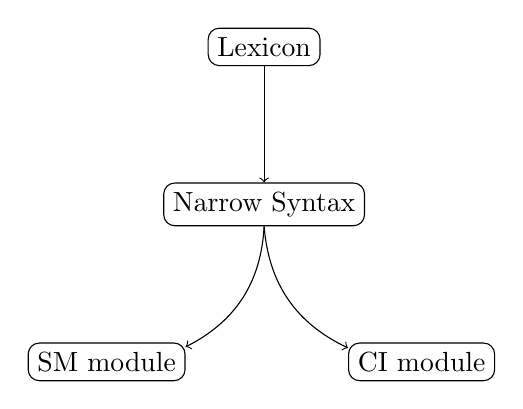
\begin{tikzpicture}
		\node[draw,rounded corners] (lex) at (0,4) {Lexicon};
		\node[draw,rounded corners] (syn) at (0,2) {Narrow Syntax};
		\node[draw,rounded corners] (sm) at (-2,0) {SM module};
		\node[draw,rounded corners] (ci) at (2,0) {CI module};
		\path[->] (lex) edge (syn)
			(syn.south) 	edge[bend left] (sm)
					edge[bend right] (ci);	
	\end{tikzpicture}
	\caption{The Y Model of the language faculty}
	\label{fig:YModel}
\end{figure}
In this model, a narrowly syntactic ``module'' operates on items drawn from a lexicon to generate structures that are evaluated by a pair of modules:
the Sensorimotor (SM) module, commonly called the morphophonology, or PF, which is responsible for external expression, and the Conceptual-Intentional (CI) module, commonly called the semantics, or LF, which is responsible for interpreting structures for use in internal systems of thought.
Beyond this, there is significant disagreement among minimalist theorists.

Another assumption common to minimalist syntacticians is the syntactic operation Merge.
The primary (and, in some theories, only) syntactic operation, Merge combines pairs of syntactic objects (\textit{i.e.}, lexical items or syntactic structures) to form larger syntactic objects.
The standard formulation of Merge is given in \cref{ex:MergeStd}\footnote{
	\textcite{hornstein2009theory} departs from the standard formulation, defining Merge as concatenation rather than set formation.
}.
\ex.\label{ex:MergeStd} Merge$(\alpha, \beta) = \left\{ \alpha, \beta \right\}$\\
iff both $\alpha$ and $\beta$ are syntactic objects.

Merge is responsible not only for creating new structures, but also for syntactic displacement.
To my knowledge this ability was discovered by \textcite{chomsky2004beyond} when he distinguished between the two logically possible cases of Merge: external and internal.
An instance of Merge$(\alpha, \beta)$ is external if neither $\alpha$ nor $\beta$ contains the other, and internal if $\alpha$ contains $\beta$ or vice versa.
Both cases, of course, create a new object, but in the case of internal Merge, the operation has the effect of creating displacement as shown in \cref{ex:IntMerge}.
\ex.\label{ex:IntMerge} Merge$(\alpha, \{\ldots\alpha\ldots\}) = \{\alpha, \{\ldots\alpha\ldots\}\}$

Again, beyond the basics discussed above, there is little consensus among minimalist syntacticians about the nature and operation of Merge.

While the Y Model and Merge seem to be the only instances of true consensus among minimalist syntacticians, there is growing agreement about the underlying representation of certain types of word.
Specifically, many minimalist syntacticians now assume that a lexical word, like the noun \textit{chair}, minimally consists of an acategorial root and a categorizing head \parencite{borer2005name,marantz1997no}.
This is commonly expressed in the formalism of a vocabulary insertion rule from the theory of Distributed Morphology as in \cref{ex:VIRule}.
\ex.\label{ex:VIRule} \textit{chair} $\leftrightarrow \left\{ n, \sqrt{\textsc{chair}} \right\}$

There are competing views of the syntactic nature of morphological words, but as of this dissertation's writing this is a standard view, a view to which I subscribe, and therefore, I will not explicitly argue for it.

The theory I assume is not entirely standard, though.
There are a number of assumptions that I make, which will certainly raise the eybrows of many if not most contemporary syntacticians.
I discuss these assumptions in \cref{sec:nonstandard}.

\subsection{Minimalism and the Strong Minimalist Thesis}
The minimalist program can be viewed as an effort to simplify Government and Binding theory without losing its empirical coverage.
That is, a minimalist analysis is one that compares two hypotheses that have roughly equivalent empirical power, and chooses the simpler one.
However, as \textcite{chomsky1965aspects} discusses, there is no such thing as an absolute measure of simplicity.
Consider, for instance, the following equivalent expressions of arithmetic using the more standard infix notation in \cref{ex:StdAddition} and lambda calculus in \cref{ex:ChurchAddition}.
\ex.\label{ex:StdAddition} $3 + 2$

\ex.\label{ex:ChurchAddition} $\lambda f \lambda x . ((\lambda f \lambda x . f(f(f x))) f(\lambda f \lambda x . (f(f x))(f x)))$

While it may seem obvious that \cref{ex:StdAddition}, which consists of a mere three symbols, is simpler than \cref{ex:ChurchAddition} with its 41 characters, it becomes less obvious when we compare as wholes, the systems that they are drawn from.
Performing arithmetic with infix notation requires rote memorization of the results of single digit addition, multiplication, subtraction, and division, and rather complex algorithms for larger numbers (\textit{e.g.}, long division).
The lambda calculus, on the other hand, uses two very simple operations---$\alpha$-conversion and $\beta$-reduction---requiring no rote memorization for their application.
From this standpoint the lambda calculus is vastly simpler.
The point here is that a judgment of simplicity depends on the choice of simplicity metric.

This is not to say that the choice of simplicity metric is arbitrary.
On the contrary, since any choice of simplicity metric will be a major factor in deciding between theories, that choice must be justified.
The main simplicity metric of the minimalist program is the Strong Minimalist Thesis (SMT) which states that the language faculty is an optimal solution to interface conditions \parencite{chomsky2001derivation}.
One of the justifications for SMT, often repeated by Chomsky, comes from evolutionary biology.
It begins with two observations, the results of several decades of linguistics research.
The first observation is that the human language faculty is unique in the biological world, that ``nothing does language like we do,'' to use Norbert Hornstein's oft-repeated formulation.
The second observation is that the language faculty is uniform across our species, that a child born in a remote African village, but raised in Dublin would acquire an Irish variety of English with the same ease as a child born and raised in Dublin.
These observations suggest that the language faculty emerged quite suddenly, likely due to a single genetic mutation in a single individual.
It follows from this that whatever portion of our cognitive system that is specific to language must be very simple.

The SMT provides the following principles for minimalist syntactic analysis and theorizing:
\begin{enumerate}[noitemsep]
	\item Assume the simplest possible recursive syntax (\textit{i.e.}, one that consists only of simplest Merge).
	\item Assume that no other module of the language faculty is capable of recursion.
	\item When you encounter a proposed property of the language faculty or principle of linguistic theory either 
		\begin{enumerate}[noitemsep]
			\item show that it can be reduced to Merge,
			\item show that it can be reduced to interface conditions,
			\item show that it can be reduced to independent principles, or
			\item show that it can be reduced to a combination of Merge, interface conditions, and independent principles.
		\end{enumerate}
	\item It is only when we can show that any such reduction is impossible that we may modify our assumptions.	
\end{enumerate}

One might object that this places an unreasonable burden on linguists.
The principles, however, follow from the basic principles of science, and they are inapplicable to the study of human language only insofar as human language is immune to scientific inquiry.
So, to abandon these principles at the first sight of difficulty is to abandon the scientific approach to understanding the language faculty.
\end{document}                                                                                            
